%20 min preso!
\documentclass[xcolor=table]{beamer}
\usepackage{beamerthemesplit}
\usepackage{wrapfig}
\usetheme{SPbGU}
\usepackage{pdfpages}
\usepackage{amsmath}
\usepackage{cmap}
\usepackage[T2A]{fontenc}
\usepackage[utf8]{inputenc}
\usepackage[english]{babel}
\usepackage{indentfirst}
\usepackage{amsmath}
\usepackage{tikz}
\usepackage{multirow}
\usepackage[noend]{algpseudocode}
\usepackage{algorithm}
\usepackage{algorithmicx}
\usepackage{fancyvrb}
\usepackage{verbatim}
\usetikzlibrary{calc}
\usetikzlibrary{shapes,arrows}
\usetikzlibrary{arrows,automata}
\usetikzlibrary{positioning}

\usepackage{tabularx}
\newcolumntype{Y}{>{\raggedleft\arraybackslash}X}

\renewcommand{\thealgorithm}{}

\newtheorem{mytheorem}{Theorem}
\renewcommand{\thealgorithm}{}

\newcommand{\tikzmark}[1]{\tikz[overlay,remember picture] \node (#1) {};}
\def\Put(#1,#2)#3{\leavevmode\makebox(0,0){\put(#1,#2){#3}}}

\newcommand{\ltz}{$< 1$}


\tikzset{
    state/.style={
           rectangle,
           rounded corners,
           draw=black, very thick,
           minimum height=2em,
           inner sep=2pt,
           text centered,
           },
}

\beamertemplatenavigationsymbolsempty

\title[Formal grammars + Neural Networks]{ON SECONDARY STRUCTURE ANALYSIS BY USING
FORMAL GRAMMARS AND ARTIFICIAL NEURAL
NETWORKS}
%\subtitle[YaccConstructor]{Parsing techniques for graph analysis}
% То, что в квадратных скобках, отображается в левом нижнем углу.
\institute[]{
JetBrains Research, Programming Languages and Tools Lab  \\
Saint Petersburg University
}

% То, что в квадратных скобках, отображается в левом нижнем углу.
\author[Polina Lunina]{Semyon Grigorev, \textbf{Polina Lunina}}

\date{September 6, 2019}

\begin{document}
{
\begin{frame}[fragile]
  \begin{table}
  \centering
  \begin{tabularx}{\linewidth}{YcX}
    
\includegraphics[height=1.5cm]{pictures/jetbrainsResearch.pdf} \hfill
    & \begin{minipage}[t]{0.3\textwidth}\center \vspace{-1cm}  CIBB 2019
      \end{minipage}
    & \hfill 
\includegraphics[height=1.5cm]{pictures/SPbGU_Logo.png}
  \end{tabularx}
  \end{table}
  \titlepage
\end{frame}
}

\begin{frame} \frametitle{Genomic sequences analysis}
\begin{itemize}
    \item Secondary structure handling
    \begin{itemize}
        \item Covariance models
        \item Hidden Markov Models
        \item Probabilistic grammars
    \end{itemize}
    \item Probability estimation for noisy data processing
        \begin{itemize}
        \item Covariance models
        \item Probabilistic grammars
        \item Neural networks
    \end{itemize}
\end{itemize}
\end{frame}

\begin{frame}<1-2>[label=again]{Proposed solution: the earlier ideas}
Our previous work: 
\emph{S. Grigorev, P. Lunina} ``The Composition of Dense Neural Networks and Formal Grammars for Secondary Structure Analysis''
\vspace{0.5cm}
\begin{itemize}
   \item \textbf<2>{Context-free grammar to encode only basic secondary structure features}
    \begin{itemize}
        \item Recursive compositions of stems
        \item Conventional base pairing
    \end{itemize}
    \item \textbf<3>{Parsing for these features extraction}
    \begin{itemize}
        \item Matrix-based parsing algorithm 
        \item Parsing result for sequence $w$ and nontermianl $N$ is a boolean matrix $M_N$, where $M_N [i,j] = 1$, iff $w[i,j-1]$ is derivable from $N$
    \end{itemize}
    \item \textbf<4>{Neural network to solve a given sequences analysis task}
        \begin{itemize}
        \item Input: parsing result linearized and compressed into a byte vector
        \item Dense and dropout layers with batch normalization 
    \end{itemize}
\end{itemize}
\end{frame}

\begin{frame}[fragile] \frametitle{Grammar}
\begin{verbatim}
s1: stem<s0>
any_str: any_smb*[2..10]
any_smb: A | U | C | G
stem1<s>:               \\ stem of height exactly 1
      A s U | U s A | C s G | G s C
stem3<s>:               \\ stem of height exactly 3
      stem1< stem1< stem1<s> > >
stem<s>:                \\ stem of height 3 or more
      A stem<s> U
    | U stem<s> A
    | C stem<s> G
    | G stem<s> C
    | stem3<s>
s0: any_str | any_str stem<s0> s0
\end{verbatim}
\end{frame}

\addtocounter{framenumber}{-2}
\againframe<3>{again}
\addtocounter{framenumber}{1}

\begin{frame}{Example}
\centering
 \texttt{CCCC{\color{red}ATTGCCAAGG}ACCCCA{\color{red}CCTTGGCAAT}CCC}
\vspace{1cm}

\tikzmark{xx}{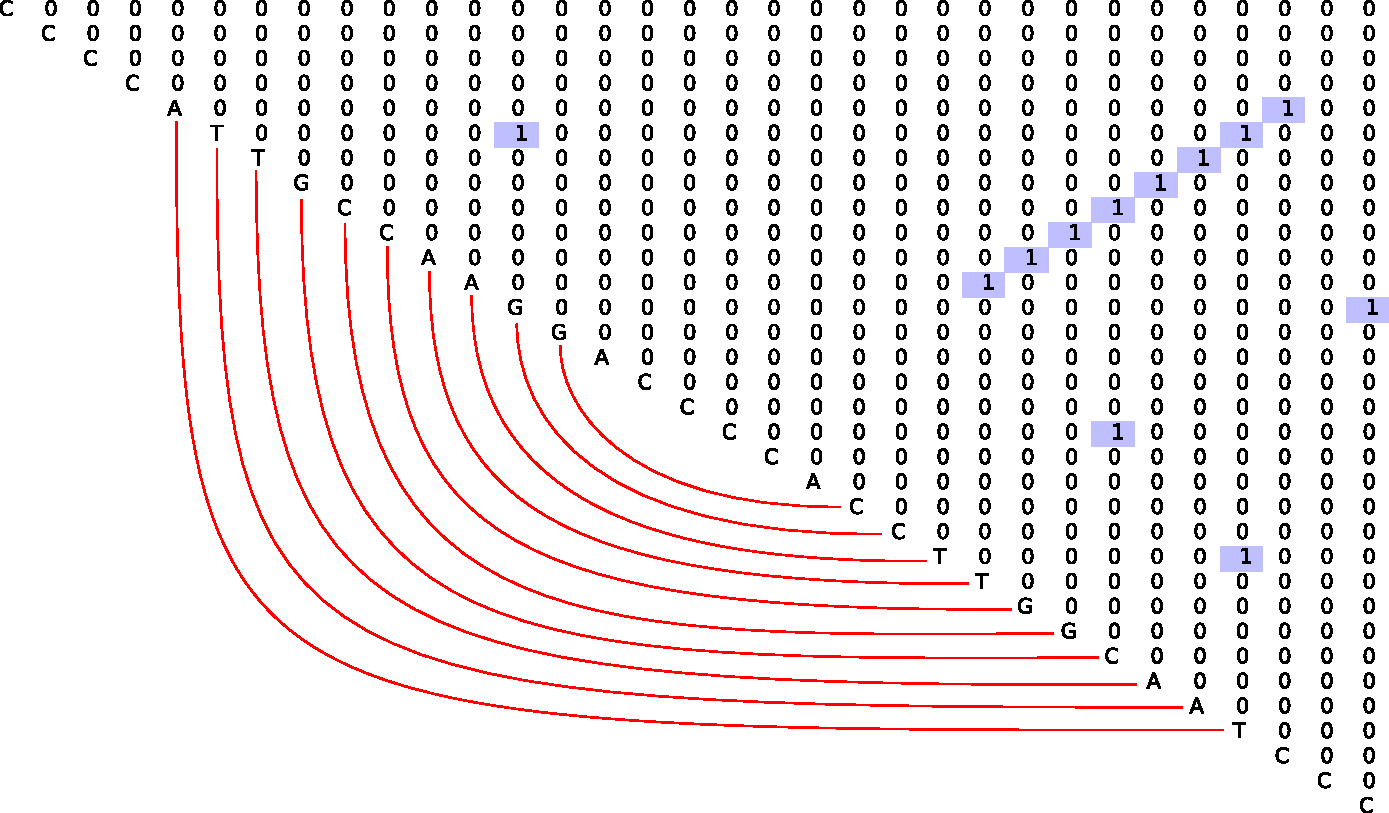
\includegraphics[width=.8\textwidth]{pictures/mtrx.pdf}}
\onslide<2-3>{
\tikz[overlay,remember picture]{
\draw[draw=red,thick,fill opacity=0.2] ($(xx) + (1.1,4.97)$) rectangle ($(xx) + (9.05,3.235)$);
}
}

\onslide<3>{
\tikz[overlay,remember picture]{
\draw[draw=red,thick,fill opacity=0.2] ($(xx) + (5.8,4.97)$) rectangle ($(xx) + (8.75,0.4)$);
}
}
\end{frame}

\addtocounter{framenumber}{-3}
\againframe<4>{again}
\addtocounter{framenumber}{2}

\begin{frame}{Improvements (1)}
    \textbf{Problem:} vectorization breaks data locality which increases network learning time
    
 \vspace{0.3cm}   
    \textbf{Solution:}
    \begin{itemize}
        \item Represent parsing result as an image
        \item Use convolutional layers for these images processing
        \item Compare image- and vector-based networks on the same data
    \end{itemize}
\end{frame}

\begin{frame}{Parsing results representation}
\tiny %\hspace{-2cm}
  \begin{tikzpicture}[->,>=stealth']

  \node[state,
        align = left,
        text width = 5.5cm] (mtrx)
  {
    \textbf{Matrices}\\
    %\vspace{0.05cm}
    \[ \left( \begin{array}{ccccc}
    0 & 1 & 0 & ... & 1\\
    0 & 0 & 1 & ... & 0\\
    0 & 0 & 0 & ... & 1\\
    ... & ... & ... & ... & ...\\
    0 & ... & ... & ... & 0
    \end{array} \right)\]
    \vspace{-0.1cm}

  Parsing result is a boolean matrix~$M$ which represents secondary structure features for sequence $\omega$: $ M[i,j] = 1 \iff \text{\ttfamily{s1}} \xrightarrow{*}{} \omega[i,j]$, and $0$ otherwise.
  };

  \node[state,
        right of=mtrx,
        node distance=6.5cm,
        align = left,
        text width = 5.5cm](vector)
  {
  \textbf{Vectors}\\
  \vspace{-0.1cm}


$$\texttt{[1,0,...,1,1,...,0,...,1,...]}$$
\vspace{-0.35cm}
$$\Downarrow$$
\vspace{-0.35cm}
$$\texttt{[84,128,...]}$$
%\vspace{-0.1cm}
  Line-by-line compressed matrix representation: sequence of 8 cells (bits) is compressed into a byte. Bottom left triangle of the matrix is always empty, so can be ignored. Requires the equal length of the input sequences and breaks the data locality.
  };

\node[state,
      line width=0.5mm,
      below = 1 of mtrx,
      node distance=3cm,
      align = left,
      text width = 5.5cm](image)
{
\textbf{Images}\\
\vspace{-0.2cm}
\begin{center}
\fbox{
\includegraphics[width=1.5cm]{pictures/bmp.png}}
\end{center}
The false bits of the matrix are represented as white pixels and the true bits as black ones. This approach makes it possible to process sequences of different lengths since the images can be transformed to a specified size. Data locality is preserved.

};


  \path 
   (mtrx) edge (vector)
   (mtrx.south) edge (image.north)
   ;

  \end{tikzpicture}
\end{frame}

\begin{frame}{Improvements (2)}
    \textbf{Problem:} parsing is a time-consuming operation which complicates the use of trained models
 
 \vspace{0.3cm}   
    \textbf{Solution:}
    \begin{itemize}
        \item Create a network which handles initial sequences
        \item Use two-staged learning
        \begin{itemize}
            \item Train network that takes images or vectors as an input and performs classification according to a given problem
            \item Extend it by a number of input layers that take the initial nucleotide sequence as an input and convert it to the parsing result which is handled by the pretrained layers
        \end{itemize}
    \end{itemize}
\end{frame}

\begin{frame}{Neural networks}
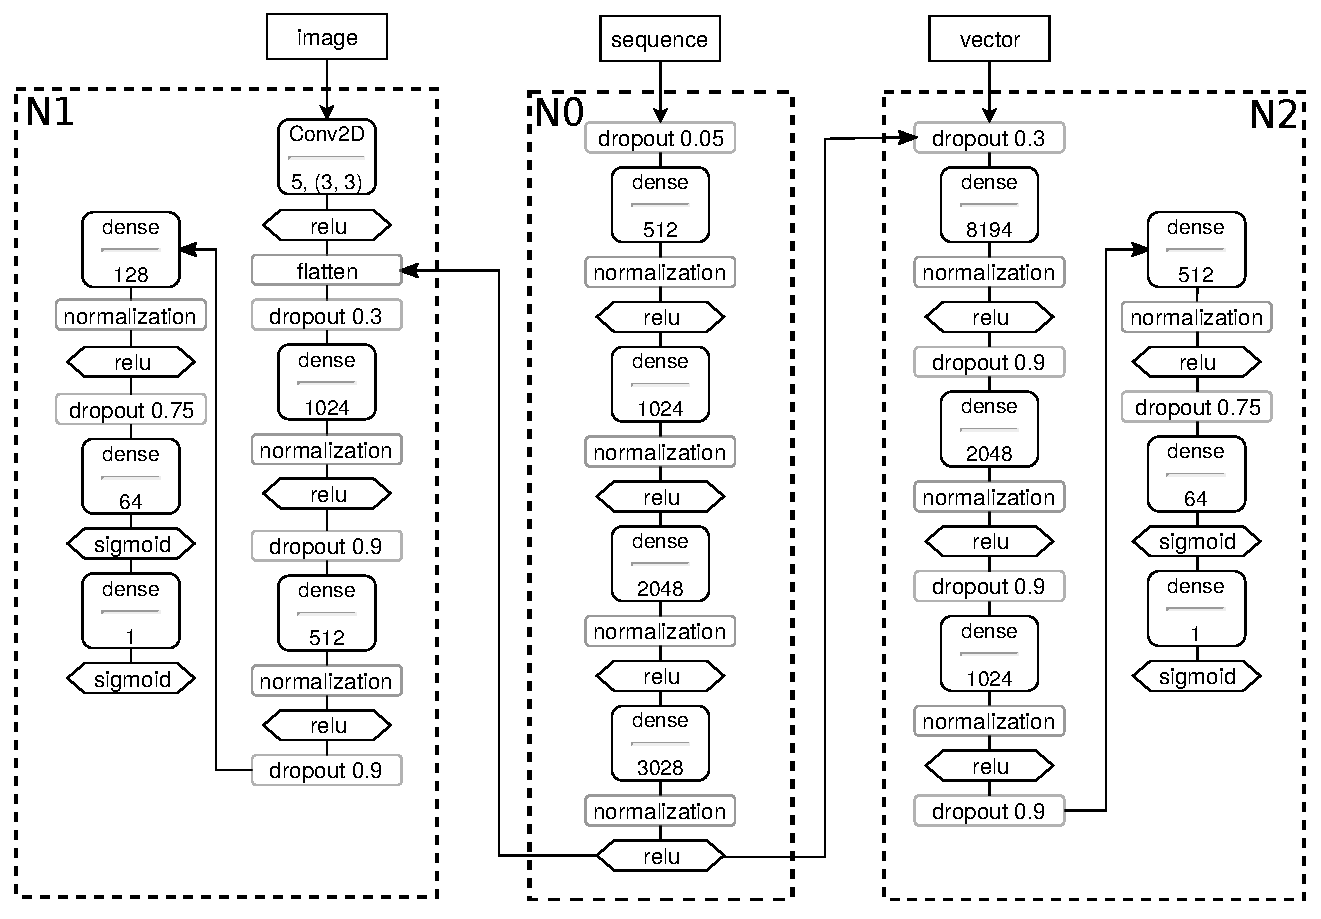
\includegraphics[width=11.5cm]{pictures/nn_arch.pdf}
\end{frame}

\begin{frame}{Final solution structure}
\begin{tikzpicture}[->,>=stealth']

  \node[state,
        line width=0.5mm,
        align=left,
        text width = 1.9cm] (grm)
   {
    \textbf{Grammar}
   };

  \node[state,
        line width=0.5mm,
        below of=grm,
        node distance=1.2cm,
        align = left,
        text width = 1.9cm] (sqs)
   {
   \textbf{Sequences}
   };

\node[state,
      double,
      draw =gray,
      line width=0.5mm,
      align = left,
      right of = grm,
      node distance = 3cm,
      text width = 1.25cm](parser)
{
\textbf{Parser}\\
};

\node[state,
      line width=0.5mm,
      right of=parser,
      node distance=3cm,
      align = left,
      text width = 1.6cm] (mtrx)
{
  \textbf{Matrices}\\
};

\node[state,
      line width=0.5mm,
      right of=mtrx,
      node distance=3cm,
      align = left,
      text width = 1.5cm](vector)
{
\textbf{Vectors}\\
};

\node[state,
      line width=0.5mm,
      below of = vector,
      node distance=1.2cm,
      align = left,
      text width = 1.5cm](image)
{
\textbf{Images}\\
};

\node[state,
      double,
      draw =gray,
      line width=0.5mm,
      below left = 1.4 and -2.2 of image,
      align = left,
      text width = 3.2cm](NN1)
{
\textbf{Neural Network 1}\\
Handles parsing results
};

\node[state,
      double,
      draw =gray,
      line width=0.5mm,
      left of = NN1,
      node distance = 6cm,
      align = left,
      text width = 3.2cm](NN2)
{
\textbf{Neural Network 2}\\
Handles nucleotide sequences
};

\node[state,
      line width=0.5mm,
      below of = NN2,
      node distance = 2cm,
      align = left,
      text width = 3.7cm](res)
{
\textbf{Classification Result}\\
};




\path (grm.east) edge (parser.west)
    (parser.east) edge (mtrx.west)
    (mtrx.east) edge (vector.west)
    (NN1.west) edge node[el,above]  {$weights$} (NN2.east)
    (NN2.south) edge (res.north);
\draw (mtrx.south) -- (6.0,-1.2) -- (image.west);
\draw (sqs.east) -- (3.0,-1.2) -- (parser.south);
\draw (vector.east) -- (11.15,0.0) -- (11.15, -4.07) -- (NN1.-12);
\draw (image.east) -- (10.8,-1.2)-- (10.8,-3.35) -- (NN1.12);
\draw (sqs.south) -- (-0.0,-3.71) -- (NN2.west);

\end{tikzpicture}

\end{frame}

\begin{frame}{Evaluation}
\begin{itemize}
    \item tRNA sequences analysis tasks
    \begin{itemize}
        \item Classification into two classes: eukaryotes and prokaryotes
        \item Classification into four classes: archaea, bacteria, plants and fungi
    \end{itemize}
    \item Tools
    \begin{itemize}
        \item Parsing: YaccConstructor platform
        \item Neural networks: Keras, Tensorflow
    \end{itemize}
    \item Databases
    \begin{itemize}
        \item tRNADB-CE
        \item Genomic tRNA database
    \end{itemize}
\end{itemize}
\end{frame}

\begin{frame}{Results}
\begin{table}[h]
\centering
\caption{Base and extended models test results by accuracy metrics}
\begin{tabular}{|l||l|l||l|l|}
\hline
Classifier                                                               & \multicolumn{2}{l||}{EP}               & \multicolumn{2}{l|}{ABFP}           \\ \hline \hline
Approach                                                                 & Vector-based       & Image-based      & Vector-based      & Image-based     \\ \hline
\begin{tabular}[c]{@{}l@{}}Base model\\ accuracy\end{tabular}            & 94.1\%             & 96.2\%           & 86.7\%            & 93.3\%          \\ \hline
\begin{tabular}[c]{@{}l@{}}Extended model \\ accuracy\end{tabular}       & 97.5\%             & 97.8\%           & 96.2\%            & 95.7\%          \\ \hline
\begin{tabular}[c]{@{}l@{}}Total training \\ time\end{tabular}       & 30000s             & 4600s           & 31800s            & 3600s          \\ \hline
\begin{tabular}[c]{@{}l@{}}Samples for\\ train:valid:test\end{tabular} & \multicolumn{2}{l||}{\begin{tabular}[c]{@{}l@{}}20000:5000:10000\\ (57\%:14\%:29\%)\end{tabular}} & \multicolumn{2}{l|}{\begin{tabular}[c]{@{}l@{}}8000:1000:3000\\ (67\%:8\%:25\%)\end{tabular}} \\ \hline
\end{tabular}
\label{acc}
\end{table}


\begin{table}[h]
\scriptsize
\centering
\begin{tabular}{|l||l|l|l|l|l|}
\hline
\multirow{2}{*}{Classifier} & \multirow{2}{*}{Class} & \multicolumn{2}{l|}{Vector-based approach} & \multicolumn{2}{l|}{Image-based approach} \\ \cline{3-6} 
                            &                        & precision         & recall        & precision        & recall        \\ \hline \hline
\multirow{2}{*}{EP}         & prokaryotic            & 95.8\%            & 99.4\%        & 96.2\%           & 99.4\%        \\ \cline{2-6} 
                            & eukaryotic             & 99.4\%            & 95.6\%        & 99.4\%           & 99.5\%        \\ \hline \hline
\multirow{4}{*}{ABFP}       & archaeal               & 91.1\%            & 99.2\%        & 91.6\%           & 98.5\%        \\ \cline{2-6} 
                            & bacterial              & 96.6\%            & 95.1\%        & 95.2\%           & 95.5\%        \\ \cline{2-6} 
                            & fungi                  & 98.5\%            & 94.9\%        & 97.5\%           & 94.3\%        \\ \cline{2-6} 
                            & plant                  & 99.4\%            & 95.7\%        & 99.2\%           & 94.7\%        \\ \hline
\end{tabular}
\end{table}
\end{frame}

\begin{frame}{Conclusion}
\begin{itemize}
    \item We propose some modifications of our approach for biological sequences analysis
    \begin{itemize}
        \item Parsing result in a form of image can be handled by convolutional layers and it decreases training time
        \item It is possible to remove the parsing step from the trained model use which allows to run models on the original RNA sequences        
    \end{itemize}
    \item These modification improve the performance of the solution and are applicable for real-world problems
\end{itemize}
\end{frame}

\begin{frame}{Future work}
\begin{itemize}
    \item Other RNA sequences analysis tasks
    \begin{itemize}
        \item 16s rRNA classification
        \item Chimeric sequences filtration
    \end{itemize}
    \item Secondary structure prediction by using generative networks
    \item Proteomic sequences processing
\end{itemize}

\end{frame}

\begin{frame}
\frametitle{Contact Information}
\begin{itemize}
  \item Semyon Grigorev:
    \begin{itemize}
      \item \href{mailto:s.v.grigoriev@spbu.ru}{s.v.grigoriev@spbu.ru}
      \item \href{mailto:Semen.Grigorev@jetbrains.com}{Semen.Grigorev@jetbrains.com}
    \end{itemize}
  \item Polina Lunina: \href{mailto:lunina\_polina@mail.ru}{lunina\_polina@mail.ru}
  \item Implementation: \href{https://github.com/LuninaPolina/SecondaryStructureAnalyzer}{https://github.com/LuninaPolina/SecondaryStructureAnalyzer}
\end{itemize}
\vspace{0.3cm}
\center{\huge{Thanks!}}
\end{frame}
\end{document}
